% =====================================================================
%  博士科研计划书 —— 面向聚变堆复杂几何的体素化特征线中子输运与GPU并行加速方法研究
%  版本：V5.3（批注修订）（2026-11-09）
%  编译：xelatex main.tex  ×2（生成目录与交叉引用）
% =====================================================================
\documentclass[UTF8, zihao=-4, fontset=none, a4paper]{ctexart}

\usepackage{fontspec}
\setmainfont{Times New Roman}
\setsansfont{Helvetica}
\setCJKmainfont{Songti SC}[AutoFakeBold=2.2, AutoFakeSlant=0.2]
\setCJKsansfont{Heiti SC}[AutoFakeBold=2.2]
\setCJKmonofont{Songti SC}
\newCJKfontfamily\songti{Songti SC}
\newCJKfontfamily\heiti{Heiti SC}
\newCJKfontfamily\fangsong{Songti SC}
\newCJKfontfamily\kaishu{Songti SC}

\usepackage[a4paper, top=2.6cm, bottom=2.6cm, left=2.7cm, right=2.7cm]{geometry}
\usepackage{amsmath, amssymb}
\usepackage{graphicx}
\usepackage{booktabs}
\usepackage{longtable}
\usepackage{etoolbox}
\usepackage{needspace}
\usepackage{array}
\usepackage{calc}
\usepackage{caption}
\usepackage{fancyhdr}
\usepackage{enumitem}
\usepackage[hidelinks, bookmarksnumbered, bookmarksopen]{hyperref}

% ---------------- 版式 ----------------
\linespread{1.42}
\setlength{\parskip}{0.35em}
\setlength{\parindent}{2em}

\pagestyle{fancy}
\fancyhf{}
\fancyfoot[C]{\zihao{-5}\thepage}
\renewcommand{\headrulewidth}{0pt}

% 章标题：第一章 / 节标题：1.1 （自动编号，与原文手工编号一致）
\ctexset{
  section = {
    name       = {第,章},
    number     = \chinese{section},
    format     = \centering\zihao{3}\bfseries,
    beforeskip = 1.2ex plus .2ex,
    afterskip  = 2.2ex plus .2ex,
  },
  subsection = {
    format     = \zihao{4}\bfseries,
    beforeskip = 1.8ex plus .3ex,
    afterskip  = 1.0ex plus .2ex,
  },
}
\renewcommand{\thesubsection}{\arabic{section}.\arabic{subsection}}

% 图表标题
\captionsetup{font=small, labelsep=quad, skip=6pt}
\captionsetup[longtable]{font=small, labelsep=quad, skip=4pt}
\AtBeginEnvironment{longtable}{\small}
\newcommand{\tabnote}[1]{\par\noindent{\footnotesize #1\par}}

% ---------------- 自定义命令 ----------------
% 上标数字引文，例如 \upcite{1,2} -> [1,2]
\newcommand{\upcite}[1]{\textsuperscript{[#1]}}

\graphicspath{{figures/}}

% =====================================================================
\begin{document}

% ---------------- 封面 ----------------
\begin{titlepage}
  \centering
  \vspace*{2.4cm}
  {\zihao{2}\bfseries 博士科研计划书\par}
  \vspace{1.6cm}
  {\zihao{3}\bfseries 面向聚变堆复杂几何的体素化特征线\\[0.6ex]
   中子输运与GPU并行加速方法研究\par}
  \vspace{2.4cm}
  {\zihao{4} 博士学位申请 · 研究计划\par}
  \vspace{6cm}
  {\zihao{5} 版本 V5.3（批注修订）\par}
  \vspace{0.6ex}
  {\zihao{5} 2026 年 11 月 9 日\par}
  \vfill
\end{titlepage}

% ---------------- 目录 ----------------
\pagenumbering{roman}
\begingroup
\linespread{1.05}\selectfont
\setlength{\parskip}{0pt}
\tableofcontents
\endgroup
\clearpage

% ---------------- 正文 ----------------
\pagenumbering{arabic}
\setcounter{page}{1}




\section{研究背景与目标}\label{sec:1}

\subsection{聚变屏蔽的工程需求与计算问题}

聚变装置的屏蔽设计需要在有限的空间内同时满足磁体辐照、结构材料寿命、维护作业和氚增殖等要求。D-T反应产生的约14 MeV中子穿过第一壁、包层、屏蔽体与真空室后，可通过散射、俘获及次级粒子产生向外传递能量。超导磁体中的核热决定低温系统的附加热负荷，绝缘材料的辐照影响磁体寿命，维护区域的剂量则影响设备布置与作业安排。输运计算把几何、材料和核反应数据联系到这些可评价的工程响应，是比较屏蔽方案的基础\upcite{1,2}。

聚变屏蔽中的复杂性首先来自材料与传播路径的三维分布。薄层屏蔽、斜交界面、诊断孔道和管线穿透件同时存在，局部结构的改变可能使中子穿过不同材料，或增加经孔道及壁面散射到达外部区域的概率。对于磁体背侧和厚屏蔽后的探测位置，响应由穿透屏蔽或经散射到达目标区域的粒子贡献。因此，几何模型既要描述部件形状，也要准确表示中子沿传播路径穿过的材料及其厚度。材料段长度与宏观总截面的乘积决定该段的光学厚度，它是衡量中子沿程碰撞与衰减的无量纲量。体素化引起的界面位移会改变材料段长度，进而影响屏蔽后的中子通量和反应率。

聚变堆屏蔽设计需要反复比较不同材料、屏蔽厚度和孔道布局。参数化建模与输运计算的联用已用于三维设计扫描\upcite{3}，但每次修改几何或材料后，都可能需要重新生成材料映射和特征线，并完成多群源迭代。三维模型中的轨迹数据量随空间与角向分辨率增加，求解时间和存储需求限制了可比较的设计方案数量。本研究将体素化材料表示与GPU特征线扫描结合，研究在满足屏蔽响应精度的条件下减少轨迹存储、改善并行负载并缩短完整输运求解时间的方法。

\subsection{中子输运问题与计算需求}

本研究以稳态多群固定源输运为主要问题。对能群\(g\)，角通量\(\psi_{g}\)在给定材料中的平衡可写为

\begin{equation}
\Omega \cdot \nabla\psi_{g} + \Sigma_{t,g}\psi_{g} = Q_{g}\lbrack\psi\rbrack + q_{g}.
\label{eq:1}
\end{equation}

其中，\(\Omega\)为运动方向，\(\Sigma_{t,g}\)为宏观总截面，\(q_{g}\)为外源，\(Q_{g}\)表示离散能群之间的散射和所纳入的次级粒子产生。源归一化、材料密度及边界条件共同确定输运问题，对空间区域\(V_{D}\)中的线性响应，可定义

\begin{equation}
R = \sum_{g}^{}{\int_{V_{D}}^{}{d_{g}(r)\phi_{g}(r)dV}},\phi_{g} = \int_{4\pi}^{}{\psi_{g}d\Omega}.
\label{eq:2}
\end{equation}

响应函数\(d_g\)由所评价的物理量确定。区域平均通量采用体积归一化权重，反应率采用相应宏观反应截面，中子剂量采用能量相关的通量--剂量转换系数。本研究以屏蔽区域的中子通量、反应率和剂量为主要响应，采用相同的物理源归一化比较不同空间离散及GPU实现的误差与计算时间。

确定论方法将空间、角度和能量离散，通过求解输运方程获得全域通量。伴随输运则提供粒子状态对指定响应的贡献，即重要性信息。蒙特卡罗方法逐个抽样源粒子的初始状态、飞行距离和碰撞反应，跟踪粒子及其后代，以计分结果的平均值估计响应。确定论与蒙卡的耦合利用近似正向或伴随场生成重要性，据此设置蒙卡源偏倚和权窗，增加对目标响应有贡献的粒子数，并通过权重修正保持响应估计的无偏性\upcite{4,5}。

\subsection{总体研究问题与目标}

本研究以体素化特征线法（MOC）与GPU并行计算为主体。研究内容包括复杂几何的体素化材料映射及特征线追踪、GPU轨迹扫描与通量求和，以及响应精度和显存约束下的网格划分与GPU计算方法的选择。

体素表示便于材料定位和局部数据访问，局部加密能够提高薄层与材料界面的分辨率，同时也会增加源区、射线交点和通量求和操作。GPU可并行处理大量轨迹与能群任务，但轨迹段数不均匀和同址通量写入会降低执行效率。因此需要研究体素分辨率如何改变轨迹段数、访存和线程负载，并据此选择网格划分与GPU计算方法，提高给定响应精度下的输运计算效率。

申请人拟参与体素化MOC程序开发，研究材料路径与响应误差、GPU扫描成本及网格与GPU参数的联合选择，形成经数值和实验基准检验的方法。快速正向或伴随场用于成熟CADIS/FW-CADIS的应用验证，中子--光子耦合作为后续扩展。

\section{复杂几何体素化与MOC空间离散研究现状}\label{sec:2}

\subsection{几何表示与材料界面处理}

输运计算中的几何表示需要回答两个问题：粒子位于哪种材料中，以及沿给定方向何时进入下一种材料。CAD通常以曲面和实体边界描述设计部件，构造实体几何（CSG）以基本曲面和布尔运算定义区域。由CAD转换为输运模型时，需要把设计实体整理为无遗漏、无重叠且材料赋值明确的空间分区。Tsige-Tamirat等利用McCad生成ITER中子学模型，用MCNP抽样估计各材料区域的体积，并与CAD模型中的对应体积比较，核对转换前后各区域的体积偏差\upcite{6}。

Chen等在SuperMC中将MCAM的CAD建模与射线求交用于二维MOC计算，并采用菱形差分处理空间近似误差\upcite{7}。射线与CAD边界相交后得到各材料段的起点和终点，段长随后用于角通量递推。该方法将几何求交直接用于特征线分段，源项近似和角向求积则分别控制段内源项及方向积分的精度。

在蒙卡方法中，DAGMC利用CAD表面的三角面元进行粒子定位与射线求交，从而直接访问CAD几何。三角面元对曲面的近似精度由面元划分及几何容差控制。Shriwise等将有符号距离场（SDF）作为下一表面求交的预筛选器：输入粒子位置、拟飞行距离及距离场误差界，如果距离场及其误差界表明粒子在下一次碰撞前不会穿过材料边界，就省去此次边界求交。存在越界可能时，仍调用DAGMC射线求交以确定交点\upcite{8}。距离场用于筛选需要求交的粒子飞行过程，实际材料边界仍由原几何追踪算法确定。表\ref{tab:1}列出同一氢球算例的时间，表明表面筛选降低了CAD查询开销，但仍保留了显式几何求交。其后，Shriwise等将Embree射线追踪内核用于CAD面元访问\upcite{9}。减少重复边界求交可以降低几何追踪开销。MOC则需要沿轨迹生成完整的材料段序列，后续源迭代还可复用这些数据。因此，空间索引在MOC中的作用需要结合段生成次数和轨迹复用次数评价。



非贴体方法使用独立于实体边界的背景网格，材料界面可以穿过网格内部。Yang等基于SALOME完成边界表示到CSG的转换，在笛卡尔和柱坐标单元中采用体积加权的材料均匀化，减少只以单元中心位置决定材料所造成的映射偏差\upcite{10}。Buchan等进一步采用supermeshing，即由实体网格与背景网格的交叠关系构造材料投影，并将守恒投影与背景有限元网格自适应结合\upcite{11}。两类方法都将几何生成与求解网格分开管理，区别在于混合材料参数及投影进入离散方程的方式。

材料体积分数和方向传播特征承担不同作用。一个含窄孔道的单元即使保持相同空隙体积分数，均匀混合后的材料也可能给沿孔道运动的粒子分配额外碰撞。沿某条特征线，各段的宏观总截面与长度之积累加为光学厚度。细薄高吸收层的位置和厚度会直接改变沿程衰减。图\ref{fig:1}将曲面、局部网格与材料段对应起来，说明材料投影需要同时核对体积、交点、弦长和通道连通性。

\begin{figure}[htbp]
\centering
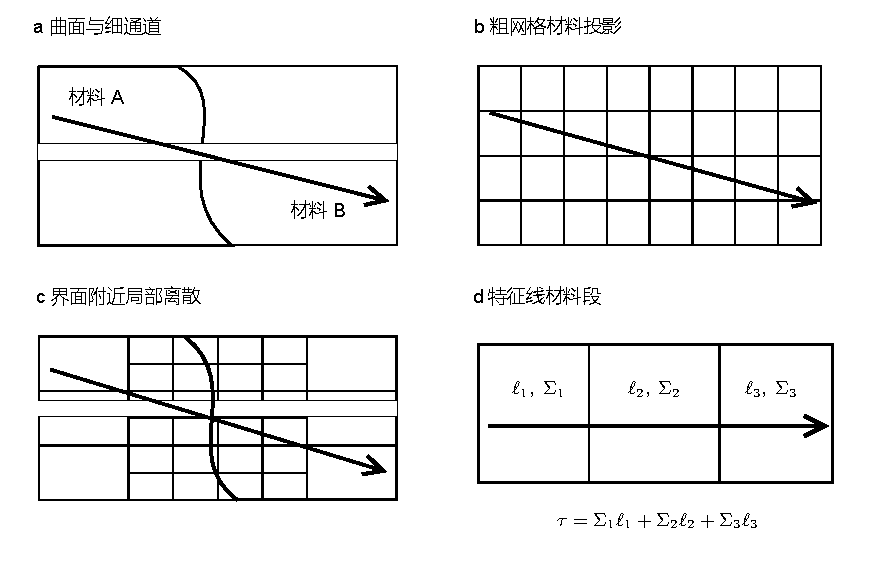
\includegraphics[width=0.95\linewidth]{figures/fig1}
\caption{非贴体材料表示与特征线分段\upcite{7,10,11,12}}
\label{fig:1}
\end{figure}



规则体素通过整数索引访问材料与源区数据，局部细化则提高指定区域的空间分辨率。块结构方法将细化单元放在矩形块内，用连续数组保存各块的数据，再由层级索引处理粗细网格的关系。AMReX中的Box、BoxArray和DistributionMapping分别描述矩形区域、块集合及其并行分配，重网格时依据标记聚类形成新块，再迁移数据\upcite{13}。GPU自适应笛卡尔网格研究还分析了相邻网格层级差异的控制、网格并行构建及动态更新所需的计算开销\upcite{14}。对中子输运，块的计算负载还与穿越特征线数量、段长分布、能群和迭代次数相联系，因此工作量估计可以超出单元数量本身。

\subsection{体素穿越与几何界面求交方法}

均匀体素的材料定位可由坐标、网格原点和步长计算整数索引。Amanatides与Woo的快速遍历算法维护射线到下一组$x,y,z$网格面的参数值及各轴的增量，每次选择最小参数并更新相应索引\upcite{15}。原文给出的基本邻格推进操作需要两次浮点比较和一次加法。在MOC中，该算法根据射线起点、方向和网格尺寸，依次确定射线经过的体素，并计算每个体素内的射线段长度。面、棱、角交点的相等参数需一致处理，防止零长度段、漏段或重复段。相邻同材料体素可共享衰减计算，但应保留源区和通量统计区的分界。采用CMFD加速时，还需单独记录粗网界面的中子流。

局部细化改变单元尺寸，均匀DDA的固定轴向增量因而不能直接贯穿所有层级。Laine与Karras用稀疏八叉树保存表面附近的体素，在每个节点记录八个子节点是否存在，并利用相对地址定位子节点，减少树结构的存储量\upcite{16}。用于中子输运时，可沿八叉树逐层定位射线穿过的叶单元，即不再细分的空间单元，并读取该单元的尺寸和材料编号。中子输运需要继续追踪穿过真空孔道和多层材料的射线，并为相应源区计算通量。八叉树用于输运时，需保留这些区间及源区信息，同时记录树节点存储、地址访问和跨层定位的计算成本。

层次包围盒（BVH）将CAD面元按空间位置分组，用逐层嵌套的包围盒建立树结构。射线追踪时，先检查射线是否与包围盒相交，排除不相交盒内的面元，再对剩余候选面元求交。随后对交点排序并判断所处实体，得到材料边界与材料编号。体素与几何界面结合的追踪方法可在界面单元中使用BVH辅助求交，在其余单元中采用规则体素穿越。图\ref{fig:2}比较体素穿越、叶单元定位和面元求交。

\begin{figure}[htbp]
\centering
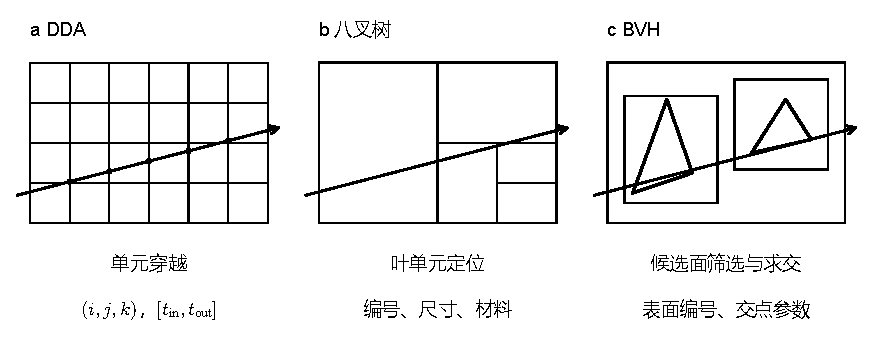
\includegraphics[width=0.95\linewidth]{figures/dda_index}
\caption{DDA、八叉树与BVH射线追踪示意}
\label{fig:2}
\end{figure}

\subsection{源项近似与源区通量积分}

MOC把指定方向的输运方程转化为沿射线的一维递推。射线与材料界面及源区边界的交点将其划分为多个段。每段需要总截面、长度和源项的近似表示。对给定能群、离散方向和源迭代步，以下将总角源\(Q_g[\psi]+q_g\)简记为\(Q\)，它是每单位立体角的源，已包含散射与外源的角向归一化。各向同性标量源\(S_g\)对应\(Q=S_g/(4\pi)\)。各向异性散射以所采用阶次的角矩重建并记录其截断阶。段内截面和\(Q\)均为常数时，出射角通量由

\begin{equation}
\psi_{out} = \psi_{in}e^{- \Sigma_{t}l} + \frac{Q}{\Sigma_{t}}(1 - e^{- \Sigma_{t}l})
\label{eq:3}
\end{equation}

给出，其中\(l\)为材料段长，\(\Sigma_{t} > 0\)。真空极限\(\Sigma_{t} \rightarrow 0\)取\(\psi_{out} = \psi_{in} + Ql\)。小光学厚度下采用稳定的指数差计算。段平均角通量及其对源区标量通量的贡献可写为
\begin{equation}
\begin{aligned}
\bar\psi_{kns}&=\frac{Q}{\Sigma_t}+\left(\psi_{\rm in}-\frac{Q}{\Sigma_t}\right)\frac{1-e^{-\tau}}{\tau},\quad \tau=\Sigma_t\ell_{kns},\\
\phi_r&\simeq\frac{1}{V_r}\sum_n w_n\sum_{(k,s)\in r}a_{kn}\ell_{kns}\bar\psi_{kns}.
\end{aligned}
\label{eq:tally}
\end{equation}
式中各量均对应同一能群，\(n,k,s\)分别表示离散方向、轨迹和轨迹子段，\(w_n\)为角权重（和为\(4\pi\)），\(a_{kn}\)为与角权重分开的射线横截面求积权重，\(V_r\)为源区体积。每个方向的轨迹横截面权重与段长之积用于近似源区体积，并按源区体积归一化得到标量通量。反应率由相应空间区内的标量通量与宏观反应截面相乘后积分得到。真空段平均值取\(\psi_{\rm in}+Q\ell/2\)，小光学厚度采用指数差或级数保持稳定。特征线需要在材料、源项近似或通量统计区域发生变化的位置分段。相邻区间即使具有相同材料和源值，也应分别计算各源区的通量积分。采用粗网有限差分（CMFD）加速时，还需记录穿过粗网界面的中子流。扫描中可共享相同区间的衰减计算，但应保留各空间区的通量积分和界面中子流，再据此更新散射源及加速方程。由此，几何交点决定材料段，源区划分决定沿程源近似，轨迹间距和角向求积决定积分分辨率。

OpenMOC包含二维CSG射线追踪、平源MOC、源迭代和粗网有限差分加速，并以C5G7和LRA问题检验本征值与功率分布\upcite{17}。Gaston等在MOCkingbird中采用非结构网格三维长特征线，使完整轨迹穿过多个计算子域，并比较预先保存分段与求解时重新分段两种方法。其全堆芯算例达到约14亿单元、12000个处理器\upcite{18}。局部细化增加射线与网格的交点，产生更多需要保存和扫描的短段。轨迹跨越计算子域时，还要传递边界角通量。因此，评价三维MOC的存储与运行时间时，需要同时统计网格单元数、轨迹段数和跨域传输量。

Porhemmat等在二维MOC中采用模块化射线追踪（Modular Ray Tracing，MRT），利用重复栅元的局部追踪结果，减少同类几何的重复求交和轨迹存储\upcite{19}。该研究比较了三种角向求积。在Legendre--Chebyshev $S_{20}$设置下，C5G7正向和伴随计算与参考$k_{\mathrm{eff}}$之差分别为$7\times10^{-6}$和$9\times10^{-6}$，16个CPU线程的加速比为6.18。模块复用以几何重复为条件，重复栅元和一般曲面孔道因而具有不同的轨迹生成与存储需求。

\subsection{局部细化与目标响应误差控制}

Liu等在多层八叉树上建立非匹配笛卡尔网格，用于离散纵标计算，随后发展了随通量解变化的预测--校正方法，利用通量形状和平衡关系计算粗细网格界面上的通量\upcite{12,20}。这些研究表明，局部加密既要生成不同尺寸的网格，也要计算粗细网格间传递的通量，并安排满足依赖关系的扫描顺序。MOC沿轨迹把上一段的出射角通量传给下一段，可据此检查粗细单元交界处是否存在漏段、重复段或通量不连续。

自适应的另一核心问题是依据什么量分配分辨率。标准误差指标强调全域解或局部梯度。目标导向方法使用伴随信息，把残差对探测器或积分响应的贡献作为加密依据。Wang与Ragusa在二维非结构三角形网格上比较高阶间断伽辽金（DG）离散的标准与目标导向自适应，讨论点通量和区域平均反应率。Lathouwers针对体与表面探测器构造含角度依赖的对偶加权残差及目标误差控制\upcite{21,22}。远端探测区的绝对通量可能很小，目标导向选择使误差控制与需要评价的响应直接对应。

Baker等在球谐角展开和空间子网格尺度有限元框架中，用子网格校正构造残差，并组合正向、伴随各向异性误差度量，针对两个单群和一个多群固定源屏蔽问题选择加密位置\upcite{23}。Goffin等把目标泛函扩展到有效增殖因子\upcite{24}。有限元或离散纵标的残差度量依赖其离散方程，MOC的误差评价则需与沿程源近似、段积分和轨迹求积对应。

Liu等的后续工作分别推进了全局与目标精度控制。2022年研究利用多层金字塔结构、空间矩比指标和扫描优化，在达到相同精度时，相对均匀细化节省60\%---80\%的计算成本。2023年研究以加权差分通量重构残差，并以DWR驱动多群固定源与临界问题的加密，在所测目标相近精度下减少超过70\%的工作量和运行时间\upcite{25,26}。在Balakovo-3固定源剂量基准中，多层八叉树将约950万网格降至190万，对传统离散纵标计算和实验结果的RMS差异分别约为4\%与10\%，相对均匀细网格节省约70\%计算成本\upcite{27}。这些结果为采用局部细化减少达到指定响应精度所需的工作量提供了依据。

近年的发展还包括提高空间阶次。Wilson等将非连续等几何离散、目标误差度量、局部\(h(p)\)细化与扩散加速结合，在参考空间求解后投影形成误差估计\upcite{28}。这使网格划分具有改变单元尺寸和提高解表示阶次两种选择。表\ref{tab:1}按数值处理与验证结果归纳代表性工作。改变单元尺寸、提高源展开阶次和重构材料界面，分别影响空间积分的不同部分。 \begin{longtable}{@{}>{\raggedright\arraybackslash}p{\dimexpr0.24\linewidth-1.5\tabcolsep\relax}>{\raggedright\arraybackslash}p{\dimexpr0.22\linewidth-1.5\tabcolsep\relax}>{\raggedright\arraybackslash}p{\dimexpr0.24\linewidth-1.5\tabcolsep\relax}>{\raggedright\arraybackslash}p{\dimexpr0.28\linewidth-1.5\tabcolsep\relax}@{}}
\caption{复杂几何与目标导向空间离散的代表性研究}\label{tab:1}\\
\toprule
工作 & 对象与离散 & 数值处理 & 验证结果及启发 \\
\midrule
\endfirsthead
\toprule
工作 & 对象与离散 & 数值处理 & 验证结果及启发 \\
\midrule
\endhead
\bottomrule
\endlastfoot
Shriwise\upcite{8} & 5 MeV点源、半径10 cm、密度1 g/cm$^3$氢球，$10^8$个源粒子 & SDF预筛选下一边界查询 & DAGMC实际运行时间由25.13 min降至7.30 min，解析CSG为2.75 min \\
Gaston\upcite{18} & 非结构网格三维MOC全堆芯 & 完整轨迹与跨域角通量传递 & 约14亿单元、12000处理器，分别统计网格单元数和轨迹存储量 \\
Porhemmat\upcite{19} & C5G7二维MOC & 模块化追踪与求积比较 & 16 CPU线程加速6.18倍，复用条件取决于几何重复性 \\
Chen，Yang\upcite{7,10} & CAD-MOC，CAD至离散纵标网格 & 通用射线求交，体积加权混合材料 & 几何边界访问与材料投影分别进入输运离散 \\
Buchan\upcite{11} & 内部实体与独立背景有限元网格 & supermeshing守恒投影并结合自适应 & 分别控制实体边界和背景求解网格的分辨率 \\
Liu 2022\upcite{25} & 多层空间矩离散 & 空间矩比指标与优化扫描 & 相同精度下较均匀细化节省60\%--80\%成本 \\
Liu 2023 DWR\upcite{26} & 三维多群固定源与临界 & 加权差分重构残差及近似伴随 & 相近目标精度下工作量和时间减少$>$70\% \\
Liu 2023 Balakovo\upcite{27} & VVER-1000固定源剂量 & 多层网格、源投影与跨界映射 & 约950万$\rightarrow$190万网格，对计算/实验RMS约4\%/10\% \\
\end{longtable}

\tabnote{注：DWR为对偶加权残差，RMS为均方根差异。}

\subsection{材料路径、源区划分与扫描工作量}

体素化将连续材料边界投影到网格上，界面位置和材料标记的改变会影响射线经过的材料及其厚度。薄层和窄孔道所占体积虽小，却可能决定中子能否到达屏蔽后的目标区域。因此，体素化精度既要考察材料体积，也要考察主要传播路径上的材料次序、段长和光学厚度。

源区划分决定段内源项的近似，并影响沿程积分的次数。射线进入不同源区时，即使材料相同，也需要分别计算各源区的通量贡献。局部细化可以减少不重要区域的单元数，同时增加细化区域中的射线交点。源区总数的减少与实际扫描段数的减少因而不是简单的比例关系。

已有目标导向自适应研究表明，按响应的重要性分配分辨率，可以减少达到给定精度所需的计算量。对体素化MOC，更值得关注的是细化位置、材料路径误差和扫描段数之间的联系：改善关键路径的材料表示能带来多大的响应精度提升，又会增加多少几何查询、源区积分和通量求和。这一关系也是选择体素网格与GPU计算方法的依据。

\section{GPU-MOC并行算法研究现状}\label{sec:3}

\subsection{轨迹生成、存储与通量求和}

GPU-MOC的并行性来自给定源项下可以分别计算的轨迹、离散方向和能群，而同一轨迹内的角通量仍需沿程递推。段长、材料编号、源区编号和边界角通量构成扫描的主要输入。预存全部分段能复用首次追踪结果，代价是每步读取段数组；在线生成减少段存储，代价是在扫描时重新定位和求交；部分缓存则在二者之间选择。Zhou等研究的部分缓存和在线生成，以及MRT利用重复模块的局部轨迹复用，分别利用了迭代复用和几何重复性\upcite{19,29}。

按式\eqref{eq:tally}对各条轨迹的段积分加权求和，可得到源区的标量通量。GPU线程分别扫描不同轨迹，它们对同一源区的通量贡献需要写入通量数组的同一位置。原子加法将读取、相加和写回作为不可分割的操作，防止并行更新时丢失部分贡献；写入过于集中时，则会增加线程等待。线程块内先计算局部和，再写入全局通量数组，可以减少全局原子加法的次数，同时需要共享内存和线程同步。NVIDIA的线程束聚合示例与CUDA指南介绍了相关实现\upcite{30,31}，计算流程见图\ref{fig:3}。

\begin{figure}[htbp]
\centering
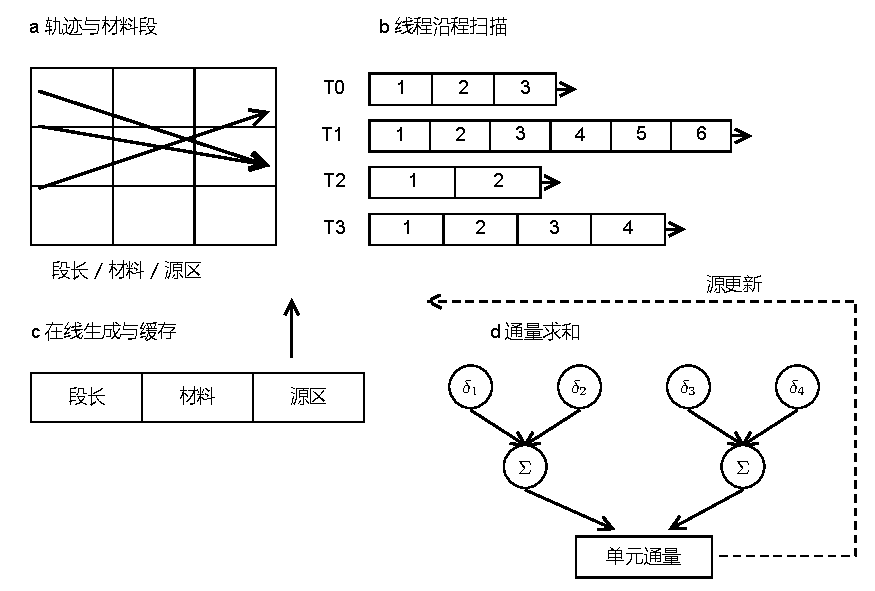
\includegraphics[width=0.95\linewidth]{figures/fig3}
\caption{GPU-MOC轨迹扫描与通量求和\upcite{29,30,32,33,34,35,36}}
\label{fig:3}
\end{figure}

\subsection{几何结构、任务分配与存储压缩}

二维OpenMOC将轨迹--能群任务分配给CUDA线程，能群内层的连续计算也用于CPU向量化\upcite{17}。在方位角从4增加到128的比较中，任务数量随角度数增加，GPU可利用的并行度提高。宋佩涛等采用通信与扫描重叠、异步传输及CPU/GPU任务分配，处理异构执行的等待\upcite{33,37}。能群并行增加同时执行的任务数，异步传输则减少计算设备等待数据的时间。

三维MOC的容量问题还取决于几何结构。Song等在平源、显式三维分段基线上结合线性源、在线轴向追踪和分批处理\upcite{32}。线性源提高源近似阶次，减少达到相应精度所需的空间分段；在线轴向追踪保存二维径向段，并利用其与轴向平面的交点构造三维段；分批处理限制同时驻留的轨迹和边界通量。一般体素几何可用DDA生成分段，但其定位和层级访问成本需要结合实际体素分布分析。

Wang等将轴向挤出几何的循环轨迹划分为比角度分解更细的任务，按估计计算量分配处理器；汪岸进一步研究周期轨迹长度与负载分配\upcite{38,39}。ANT-MOC以存储、计算和通信成本模型支持轨迹管理，并在节点、GPU和计算单元三个层次分配任务\upcite{34}。薄层、孔道和局部细化使不同轨迹的扫描段数与材料访问量产生差异，负载估计需要反映这些差异。

STREAM3D-GPU通过轴向分解降低每个MPI进程的显存驻留，并以异步执行协调计算和传输\upcite{35}。2024年KNS报告给出了逐平面传输的操作：扫描前送入入射角通量，扫描后回传出射角通量和CMFD网格界面中子流，同时保留可复用的设备数据\upcite{40}。其七群、64轴向平面C5G7在两颗EPYC 7543的64核CPU参考与同主机加8块RTX A5000之间，MOC时间由1368 s降至34 s，总时间由1704 s降至100 s；72群、197平面的OPR-1000八分之一堆芯相应为61535 s至3995 s、212416 s至11201 s。扫描与总时间的变化不同，后一算例还包含径向MPI分区等待时间的改变。

\begin{longtable}{@{}>{\raggedright\arraybackslash}p{\dimexpr0.22\linewidth-1.5\tabcolsep\relax}>{\raggedright\arraybackslash}p{\dimexpr0.25\linewidth-1.5\tabcolsep\relax}>{\raggedright\arraybackslash}p{\dimexpr0.32\linewidth-1.5\tabcolsep\relax}>{\raggedright\arraybackslash}p{\dimexpr0.21\linewidth-1.5\tabcolsep\relax}@{}}
\caption{代表性MOC并行方法的结构条件与计算结果}\label{tab:2}\\
\toprule
研究与几何对象 & 算法及利用的结构 & 实验结果与基线 & 对体素MOC的启发 \\
\midrule
\endfirsthead
\toprule
研究与几何对象 & 算法及利用的结构 & 实验结果与基线 & 对体素MOC的启发 \\
\midrule
\endhead
\bottomrule
\endlastfoot
OpenMOC\upcite{17}，二维C5G7七群 & 轨迹--能群任务，内层能群向量化 & 四种NVIDIA GPU，相对单Xeon核最大求解加速近50倍 & 角度数影响可并行任务量 \\
Song等\upcite{32}，少群三维组件/SMR & 线性源、在线轴向追踪、分批驻留 & 25 cm组件平源显式基线22129 MB；组合后组件显存降低98.5\%，可在单GPU运行四群SMR全堆芯 & 区分源阶次、段存储和驻留规模 \\
Wang等\upcite{38}，轴向挤出CPU-MOC & 循环轨迹细分与计算量分配 & 10240至98304 CPU核，并行效率$>$40\% & 根据轨迹工作量分配任务 \\
ANT-MOC\upcite{34}，三维全堆芯 & 存储/计算/通信模型，三级任务分配 & 约$10^{11}$轨迹，16000 GPU；强/弱扩展效率70.69\%/89.38\% & 容量与跨设备负载同时约束 \\
STREAM3D-GPU\upcite{35}，OPR四分之一堆芯 & 逐轴向平面处理与异步执行 & 每MPI进程约50 GB至$<$4.5 GB；8/16 GPU对128核CPU求解22.1/40.5倍 & 用驻留规模换取传输与同步 \\
NuDEAL\upcite{36}，挤出几何DGMOC & 按方位角分批，逐平面计算轴向矩 & 三维C5G7，RTX 2080 Ti；同一算例的分批比较见图\ref{fig:4} & 并发数量须结合角内任务规模 \\
\end{longtable}

NuDEAL按方位角分批扫描，以控制角通量的显存占用。其轴向挤出几何采用MOC/HFEM或DGMOC，一般多面体网格采用DFEM-$S_N$，各求解器使用不同的角通量存储和任务划分\upcite{36}。作者稿表5--6中的无控制棒三维C5G7 DGMOC算例含8507520个单元，在RTX 2080 Ti上将每批角度数由2增至32时，显存由2589 MB变为7133 MB，即原来的约2.76倍；单次输运扫描由5.25 s变为5.09 s，约缩短3.0\%；单次MOC计算时间由10.50 s变为9.21 s，约缩短12.3\%。64角全并发时显存不足。角度分批的比较见图\ref{fig:4}。

每个角度已有较多任务时，增加同批角度对扫描时间的改善较小，却会增加工作数组；单次MOC时间的变化还反映扫描以外的计算。相同框架的二维DFEM-$S_N$在RTX 4070 Ti上的顺序与并发总时间分别为148 s和26 s\upcite{36}。

\begin{figure}[htbp]
\centering
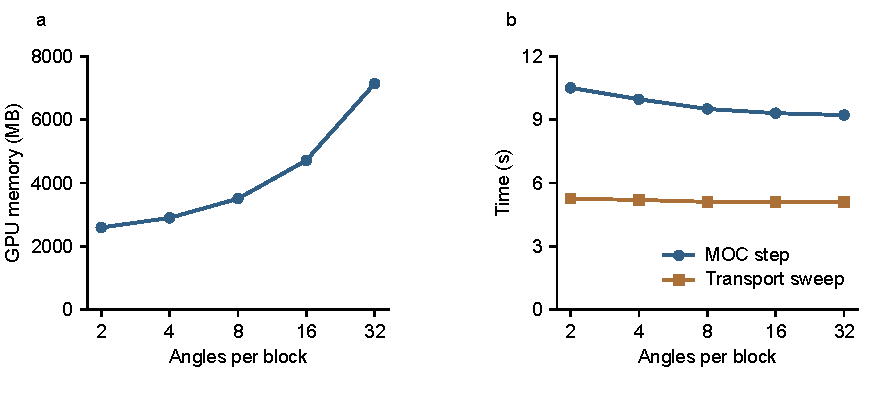
\includegraphics[width=0.95\linewidth]{figures/fig4_nudeal}
\caption{NuDEAL方位角分批对显存和计算时间的影响\upcite{36}}
\label{fig:4}
\end{figure}

\subsection{固定源扩展、伴随求解与体素离散的联系}

固定源GPU输运研究提供了不同扫描和迭代方式的参照。STRAUM采用群块Krylov和空间波前，Gong等研究三维离散纵标GPU计算\upcite{41,42}；ALPHA将全隐式瞬态固定源MOC与棒级CMFD结合，并考察单精度（FP32）计算和收敛容限\upcite{43}。Denovo的大型工程求解、OpenSn的开源实现及Pryer的批量波前计算分别涉及多维并行、可复用的程序实现和多样本任务\upcite{44,45,46}。Biondo等介绍的Shift流程则在CPU上完成Denovo正向/伴随预计算及权窗生成，在GPU上执行蒙卡输运\upcite{47}。

伴随实现还需保持离散内积关系。对实数输运矩阵\(A\)和由正体积、正求积权构成的对称正定内积矩阵\(W\)，有

\begin{equation}
A^{\dagger} = W^{- 1}A^{\mathsf{T}}W,\langle Au,v\rangle_{W} = \langle u,A^{\dagger}v\rangle_{W}.
\label{eq:4}
\end{equation}

材料和轨迹索引可以共享，散射与能群耦合需作相应转置，轨迹传播和边界交换服从配对的伴随次序。内积对偶与源--响应互易为正向--伴随实现提供检验，再将所得重要性用于第\ref{sec:4}章的混合计算\upcite{5,48}。

GPU-MOC的扫描时间取决于轨迹段数、段长分布、数据读取量以及多个线程向同一源区求和的次数。现有方法利用几何重复、轴向挤出结构或角度分批减少存储并平衡负载。体素细化和源区划分会改变这些方法面对的任务规模与分布。因此，评价复杂体素几何中的并行算法，需要将响应精度、实际扫描段数和完整求解时间联系起来。

\section{聚变屏蔽应用与数值验证依据}\label{sec:4}

\subsection{屏蔽结构、工程响应与计算需求}

聚变屏蔽中的厚材料层、薄壁部件和低密度孔道对应不同的传播条件。厚屏蔽后的响应依赖多次散射和能谱变化；孔道及穿透件则可能保留明显的方向性。磁体总核热是区域能量沉积积分，局部热功率密度需要辨认空间峰值，快中子注量和绝缘剂量具有不同的能量权重。FNS材料实验中的产氚率是特定反应率，光子加热响应（GHR）需要中子--光子耦合计算。运行中的瞬发剂量与冷却后的停堆剂量具有不同源项，后者还涉及活化和衰变过程。响应的位置、粒子类型与归一化因此决定了几何和场解需要保留哪些信息。

ITER中已有将CAD蒙卡与CADIS/FW-CADIS结合、计算线圈核热、屏蔽外剂量和通量分布的研究\upcite{49}；Denovo也用于大型聚变固定源计算\upcite{44}。CFETR线圈研究以密度降低和迭代权窗改善深穿透抽样，最终在物理密度下评价核响应；cosRMC进一步研究多层网格全局减方差\upcite{2,50}。ParaStell的参数扫描和CIT试验大厅中多维输运与近似模型的结合，分别反映了方案数量和模型求解成本对工程设计的影响\upcite{3,51}。这些应用要求快速求解既能描述主要传播路径，也能提供目标位置所需的通量或重要性分布。

\subsection{材料与孔道基准的实验依据}

SINBAD由NEA与RSICC共同维护，涵盖反应堆、聚变和加速器屏蔽实验\upcite{52}。其中FNS材料实验可检验高能中子在实体中的衰减和能谱变化，FNS-Duct则反映孔道传播及壁面散射。材料体、直通通道与折弯通道分别强调截面处理、直达流束和多次散射，适合考察不同空间及角向近似对响应的影响。

Ebiwonjumi等采用OpenMC分析FNS钨、钒和铍组件，与实验及MCNP结果比较；钨例使用Denovo/MAVRIC权窗\upcite{1}。车锐等用cosRMC计算FNS材料和孔道基准，Iwamoto等用PHITS计算铁屏蔽中的中子产额\upcite{53,54}。相关条件和结果见表\ref{tab:5}。

\begin{longtable}{@{}>{\raggedright\arraybackslash}p{\dimexpr0.2\linewidth-1.5\tabcolsep\relax}>{\raggedright\arraybackslash}p{\dimexpr0.31\linewidth-1.5\tabcolsep\relax}>{\raggedright\arraybackslash}p{\dimexpr0.22\linewidth-1.5\tabcolsep\relax}>{\raggedright\arraybackslash}p{\dimexpr0.27\linewidth-1.5\tabcolsep\relax}@{}}
\caption{聚变屏蔽基准及工程研究的条件与响应}\label{tab:5}\\
\toprule
对象与研究 & 计算方法与条件 & 响应 & 代表性结果 \\
\midrule
\endfirsthead
\toprule
对象与研究 & 计算方法与条件 & 响应 & 代表性结果 \\
\midrule
\endhead
\bottomrule
\endlastfoot
FNS钨/钒/铍\upcite{1} & OpenMC 0.14.1-dev、ENDF/B-VII.1，约14 MeV D-T源，MCNP 6.2对照 & 中子谱、反应率、TPR与GHR & 铍TPR 9点C/E：1.0295$\pm$0.1956；钨/钒GHR共7点：0.9537$\pm$0.1366 \\
FNS-Duct/FNS-W\upcite{53} & cosRMC、MCNP5及实验比较 & 中子通量谱 & 孔道传播、壁面散射及钨中能谱变化 \\
FNS铁屏蔽\upcite{54} & PHITS/JENDL-4.0 & 0.003--10 MeV积分中子产额 & 六位置C/E为1.15--1.78，原表不确定度为计数统计 \\
WISTELL-D\upcite{3} & ParaStell/\allowbreak DAGMC/\allowbreak OpenMC，99组几何，2113 MW源功率 & TBR与磁体总核热 & 厚型、增殖层占比60\%设计点：1.10、152.0 kW \\
\end{longtable}
\tabnote{注：C/E为计算值与实验值之比；TPR为产氚率；GHR为光子加热响应。$\pm$为不同测点C/E的标准差。}

FNS研究中，钒的低能中子谱、钨的部分阈反应和近源加热存在不同程度的C/E偏差\upcite{1}。按测点深度和能区比较这些偏差，有助于分析核数据、材料与源表示及探测器响应的影响。

\subsection{伴随重要性、源偏倚与目标构造}

深穿透蒙卡计算中，能够穿过屏蔽并对目标产生显著贡献的粒子很少。源偏倚改变粒子出生状态的抽样概率，分裂和俄罗斯轮盘改变后续粒子分支数量，各操作通过权重修正维持响应估计的无偏性。权窗按空间和能量区间规定适宜的粒子权重范围，近似伴随解则提供与目标响应相联系的重要性信息\upcite{4,55}。令\(L\)为线性固定源输运算子，\(q\)为物理源，\(d\)为响应函数；配对边界条件下有

\begin{equation}
L\psi = q,L^{\dagger}\psi^{\dagger} = d,R = \langle d,\psi\rangle = \langle q,\psi^{\dagger}\rangle.
\label{eq:5}
\end{equation}

内积包含空间、能量和角度积分。伴随角通量表示相应粒子状态对目标响应的期望贡献。设归一化物理源密度为\(p(x)\)，满足\(\int p(x)\,dx=1\)，\(x\)为参与偏倚的源变量。源支持集上正的重要性近似\(I(x)\)给出

\begin{equation}
C = \int_{}^{}{p(x)I(x)dx},\widehat{p}(x) = \frac{p(x)I(x)}{C},w_{0}(x) = \frac{p(x)}{\widehat{p}(x)} = \frac{C}{I(x)}.
\label{eq:6}
\end{equation}

按\(\widehat p\)抽样时以\(w_0\)修正出生权重，结果再按物理源强归一化。源偏倚和沿程权窗采用同一重要性的倒数，可使出生权重与输运中的权重控制相一致。MAVRIC的Denovo--Monaco流程及ADVANTG提供了已有实现\upcite{48,56}。

CADIS以指定响应为伴随源；FW-CADIS先计算近似正向响应，再按各目标响应的估计值调节伴随源\upcite{4,5}。对给定响应函数\(d_i\)、正估计\(\widetilde R_i\)及无量纲优先级\(\beta_i\)，归一化目标\(\sum_i\beta_iR_i/\widetilde R_i\)对应的伴随源为

\begin{equation}
d_{FW} = \sum_{i = 1}^{N_{D}}\frac{\beta_{i}}{{\widetilde{R}}_{i}}d_{i}.
\label{eq:7}
\end{equation}

较低的预估响应获得较高的伴随源权重，因而可将抽样分配到多个探测器或大范围计分。CADIS与FW-CADIS的计算流程见图\ref{fig:5}。

\begin{figure}[htbp]
\centering
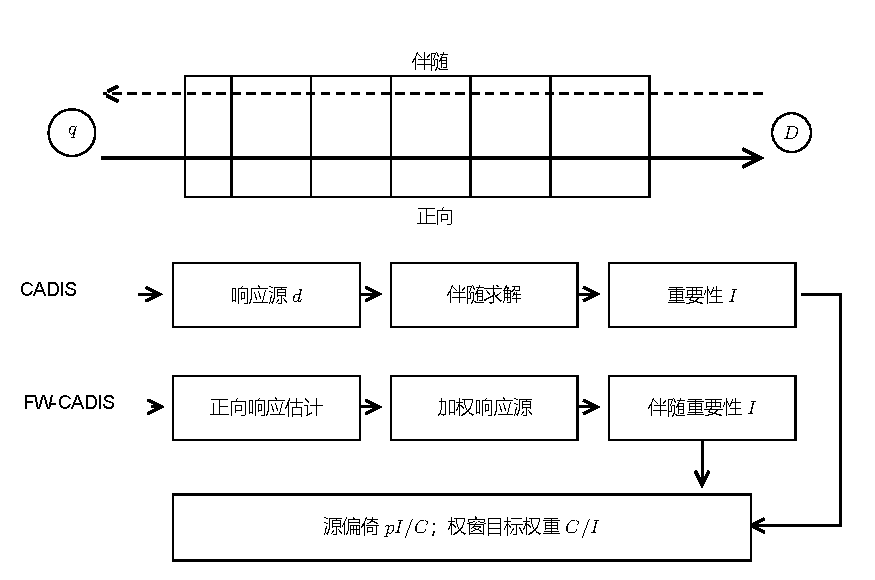
\includegraphics[width=0.95\linewidth]{figures/fig5}
\caption{CADIS与FW-CADIS重要性生成及源偏倚\upcite{4,5,48}}
\label{fig:5}
\end{figure}

方向性较强的孔道还需要考虑同一空间--能量状态中不同方向的贡献。CADIS-$\Omega$用正向角通量加权伴随角通量，定义

\begin{equation}
I_{\Omega}(r,E) = \frac{\int_{4\pi}^{}{\psi(r,E,\Omega)\psi^{\dagger}(r,E,\Omega)d\Omega}}{\int_{4\pi}^{}{\psi(r,E,\Omega)d\Omega}}.
\label{eq:8}
\end{equation}

该量在正向标量通量非零处，将实际传播方向与目标贡献联系起来\upcite{57}。LAA-CADIS以局部角度适应改进复杂通道的重要性计算\upcite{58}。MS-CADIS则针对停堆剂量，将衰变光子的目标重要性经活化过程传回中子抽样阶段\upcite{59}。

\subsection{重要性近似与完整计算效率}

重要性场既可由确定论近似解生成，也可经蒙卡迭代探索。MAGIC根据已有通量和统计信息更新权窗；随机射线方法在多群、固定源区表示下随机选取射线，迭代求正向或伴随场，可用于CADIS/FW-CADIS。OpenMC提供相应权窗生成流程\upcite{60,61}。THETA采用线性源随机射线表示单元内源变化\upcite{62}。源近似阶次影响重要性场的空间精度和存储需求。

求解重要性场的网格与蒙卡查询权窗的网格可以不同。Ibrahim等在ITER中结合材料宏观化、确定论网格细化和权窗粗化，将确定论空间--能量单元由1640万增加到5.28亿，权窗保留1630万单元\upcite{63}。相同MCNP计时和文件规模下的计分覆盖及FOM变化见表\ref{tab:4}。郑华庆等的自动网格和平滑方法，以及NECP-MCX/NECP-Hydra的正向--伴随计算与贡献粗化，分别处理重要性场求解、网格映射和权窗查询\upcite{64,65,66}。

\begin{longtable}{@{}>{\raggedright\arraybackslash}p{\dimexpr0.24\linewidth-1.5\tabcolsep\relax}>{\raggedright\arraybackslash}p{\dimexpr0.21\linewidth-1.5\tabcolsep\relax}>{\raggedright\arraybackslash}p{\dimexpr0.37\linewidth-1.5\tabcolsep\relax}>{\raggedright\arraybackslash}p{\dimexpr0.16\linewidth-1.5\tabcolsep\relax}@{}}
\caption{重要性计算与权窗输运的代表性结果}\label{tab:4}\\
\toprule
研究及算例 & 比较内容 & 文献报告值 & 对应的计算环节 \\
\midrule
\endfirsthead
\toprule
研究及算例 & 比较内容 & 文献报告值 & 对应的计算环节 \\
\midrule
\endhead
\bottomrule
\endlastfoot
ITER网格与权窗\upcite{63} & 同为10天MCNP，权窗文件约0.21 GB & 非零计分79.3\%提高到97.8\%，MC FOM提高3.4倍 & 材料宏观化、求解网格细化与权窗粗化 \\
Raffuzzi整体屏蔽\upcite{67} & 随机射线FW-CADIS，源区内常量源近似 & 只计输运时间：1.08$\pm$0.14；计入权窗生成：0.96$\pm$0.12 min$^{-1}$ & 权窗生成与生产输运的分别计时 \\
Shift先进架构\upcite{68} & CPU逐粒子输运与GPU按事件分组输运 & Frontier两例在20节点上MC运行$<$2 min，每计算芯粒（GCD）的粒子吞吐率为最佳CPU实现9--11倍 & 粒子事件分组与队列调度 \\
\end{longtable}
\tabnote{注：Raffuzzi结果为20次独立计算所得FOM的均值$\pm$标准差，单位为min$^{-1}$。}

Raffuzzi等采用源区内常量源近似，通过随机射线计算正向和伴随场，生成FW-CADIS权窗。表\ref{tab:4}分别给出只计蒙卡输运时间、以及计入权窗生成时间的FOM\upcite{67}。权窗分裂产生的大量后代可能延长少数源粒子的跟踪时间，使其他并行任务等待。Turner与Davis采用动态权窗处理这类耗时较长的粒子跟踪\upcite{69}。

对单一响应，蒙卡效率和完整应用时间可写为

\begin{equation}
{FOM}_{MC} = \frac{1}{{RSD}^{2}T_{MC}},T_{all} = T_{prep} + T_{\det} + T_{WW} + T_{MC} + T_{IO}.
\label{eq:9}
\end{equation}

其中\(RSD\)为响应估计的相对标准差，\(T_{\rm prep}\)、\(T_{\rm det}\)、\(T_{WW}\)与\(T_{IO}\)分别为准备、确定论场求解、权窗处理和输出时间；各项按不重叠的计时范围累计。全局FOM还需明确计分集合、方差汇总方式与零计分处理。由此，GPU-MOC能否改善应用效率，取决于其场解精度、预计算所占时间，以及所生成重要性对目标响应统计误差的影响。

\section{研究内容、技术路线与实施方案}\label{sec:5}

\subsection{总体研究思路与程序开发}

申请人拟在课题组已有研究基础上，参与体素化MOC程序开发，重点实现或完善几何与材料读取、体素标记、特征线穿越、源区通量积分和多群散射源迭代。先在CPU上用解析解检查材料段长和通量结果，再将同一离散计算移植到GPU，研究轨迹缓存、线程分配与通量求和。

RQ1研究体素表示与源区划分如何改变材料路径、响应误差及实际扫描工作量；RQ2固定数值离散，研究轨迹生成、存储、分组和通量求和对GPU时间与显存的影响；RQ3结合前两者，研究满足精度要求时怎样选择网格和GPU计算参数。局部细化减少的空间自由度不一定对应同比例减少的扫描段数，段数分布和地址访问又会影响线程等待与求和成本。因此，联合选择的实际效果需要与独立选择进行对照。三者的联系见图\ref{fig:cost}。

\begin{figure}[htbp]
\centering
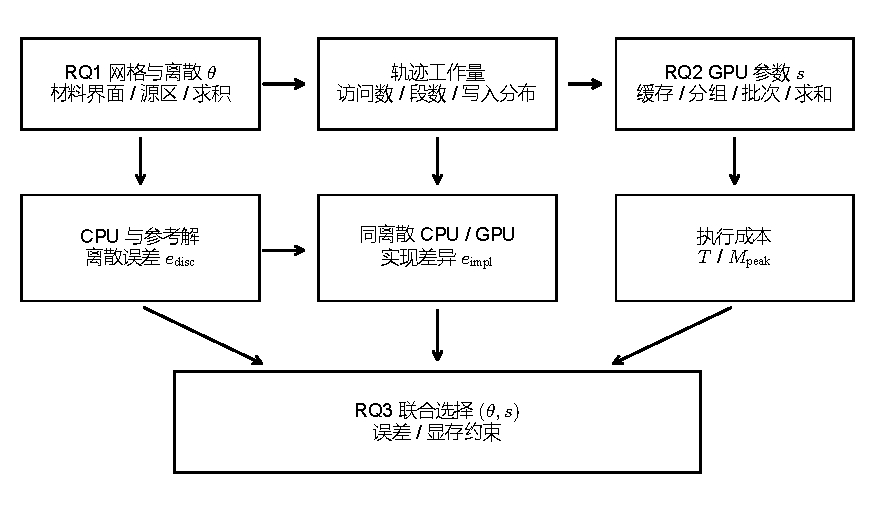
\includegraphics[width=0.95\linewidth]{figures/voxel_gpu_cost}
\caption{体素离散与GPU执行的联合优化}
\label{fig:cost}
\end{figure}

\subsection{复杂几何体素化与材料路径误差}

CAD-MOC、非贴体材料投影和层级空间离散分别提供几何求交、材料表示与局部加密的依据\upcite{7,11,12,20,25,26,27}。对薄层、斜界面和孔道，材料体积分数与沿射线的材料次序、光学厚度分别反映不同的几何信息。RQ1关注体素标记改变哪些传播路径，以及路径变化与源区近似误差如何共同影响指定响应。初步判断是：对主要贡献路径附近的细化可能比全域均匀细化更有效，但其优势取决于几何连通性、角向分辨率和新增扫描工作量。

以可解析CSG或可直接访问的CAD边界为材料参考，对相同起点和方向分别计算参考与体素材料区间，将两组交点取并集。对轨迹\(k\)、能群\(g\)，定义

\begin{equation}
\tau_{kg}=\sum_j\Sigma_{t,g,m_j}\ell_j,\qquad
\Delta\tau_{kg}=\tau^{h}_{kg}-\tau^{\mathrm{ref}}_{kg},\qquad
E_{\tau,kg}=\sum_{J}\left|\Sigma^{h}_{t,g,J}-\Sigma^{\mathrm{ref}}_{t,g,J}\right|\ell_J.
\label{eq:patherror}
\end{equation}

\(h\)表示体素网格，\(J\)为共同参数区间。\(\Delta\tau\)给出净光学厚度变化，\(E_\tau\)避免不同材料误差相互抵消。对同一正入射角通量，纯吸收无源段满足\(\psi^h_{\rm out}/\psi^{\rm ref}_{\rm out}=e^{-\Delta\tau}\)，可直接检验路径误差与出射响应的联系；散射和体源问题还需要分析源分布及方向积分。

程序开发从均匀体素与DDA开始，扩展到局部块细化和层级体素，并以界面单元直接求交作几何精度对照。中心点材料标记与子采样体积分数分别比较，混合材料采用明确的截面均匀化和源区约定。固定材料、核数据和射线集合，改变网格尺度、界面相对网格的位置及倾角、薄层厚度和孔道宽度，检查逐材料段长、光学厚度和通道连通性。

在同一映射材料模型上，独立收敛轨迹间距、角向求积、源展开和迭代，再与几何参考响应比较，可区分材料近似与输运离散的影响。按界面距离、通量变化和目标加权残差选择细化位置，比较相同时间或显存预算下的响应误差。目标导向指标借鉴已有方法\upcite{21,22,23,26}，其残差须按MOC段积分和配对伴随离散构造；初期以局部扰动响应检验灵敏度。同步统计体素数、源区数、实际扫描段数与构建成本，辨认空间误差下降而扫描工作量增加、或角向误差限制继续细化的条件。

\subsection{GPU特征线扫描与轨迹存储优化}

已有工作利用重复模块、轴向挤出结构和角度分批控制数据驻留，体现了重新计算与保存数据之间的取舍\upcite{19,29,32,34,35,36,40}。一般体素材料场中，不同射线经过的体素、材料界面和源区数量可能差异显著。RQ2研究这些差异如何改变缓存减少的重复计算量和线程等待，并识别通量求和与在线几何查询分别主导运行时间的条件。

对第\(k\)条射线，分别记录体素访问数\(N_{v,k}\)、材料段数\(N_{m,k}\)、用于源项积分的分段数\(N_{q,k}\)、按通量统计区域划分的段数\(N_{t,k}\)及实际扫描段数\(N_{s,k}\)。材料、源近似或通量统计区改变时均保留相应分界；相邻体素即使材料相同，也需分别计算各源区积分。仅在各区积分不变时共享相同区间的衰减计算，由此区分几何穿越、源项积分和通量求和各自的工作量。

GPU实现比较段长、材料编号、源区编号和轨迹偏移分别存入连续数组，与将这些量保存为结构体的方式；在同一组射线上对照全量预存、在线生成和部分缓存。缓存可按方向或空间块划分，并根据预期复用次数选择轨迹。源值改变而材料和边界不变时，几何交点可以复用；材料或源区改变则须检查段长和索引的有效范围。通过改变源迭代次数和缓存比例，分析生成、读取与重建成本的交叉点。

线程分配对照原始顺序、按段数分组和按空间位置分组。段数接近可减少短任务等待，但排序和更分散的地址访问也可能抵消这一效果。通量求和比较直接原子加法、线程块内先求和与分阶段求和，结合写入集中程度、共享内存和同步耗时解释结果。沿单条特征线始终按入射到出射的次序递推；跨设备分解时保留边界角通量传递的依赖。

纯缓存、排序和求和对照使用相同轨迹采样、源近似、求积、迭代要求和浮点精度。若策略同时改变源阶次或轨迹采样，相应参数归入数值离散，另与原离散作精度比较。除响应和守恒外，检查求和顺序引起的浮点差异。阶段计时与不启用性能分析器的重复计时配合，区分几何生成、访存、扫描、求和、传输及源更新的贡献，分析各项计算和数据传输对运行时间的影响。

\subsection{体素化与GPU执行的精度--成本协同优化}

以\(\theta\)表示材料网格、源区、轨迹采样及角向求积等数值离散参数，以\(s\)表示保持同一离散问题的缓存、线程分组、批次和求和参数。为将数值近似与实现差异分开，令\(R_{\mathrm{CPU},d}(\theta)\)为经过解析检验、守恒与收敛检查的CPU参考实现所得响应，\(R_d^{\rm ref}\)为目标物理问题的高精度参考，\(R_{\mathrm{GPU},d}(\theta,s)\)为GPU响应。联合选择写为

\begin{equation}
\begin{aligned}
e_{\rm disc}(\theta)&=\max_{d\in\mathcal D}
 \frac{|R_{\mathrm{CPU},d}(\theta)-R_d^{\rm ref}|}{a_d+|R_d^{\rm ref}|},\\
e_{\rm impl}(\theta,s)&=\max_{d\in\mathcal D}
 \frac{|R_{\mathrm{GPU},d}(\theta,s)-R_{\mathrm{CPU},d}(\theta)|}{a_d+|R_d^{\rm ref}|},\\
\min_{\theta,s}\;&T(\theta,s),\quad
 e_{\rm disc}\leq\varepsilon_{\rm disc},\quad
 e_{\rm impl}\leq\varepsilon_{\rm impl},\quad
 M_{\rm peak}\leq M_{\rm budget}.
\end{aligned}
\label{eq:joint}
\end{equation}

\(\mathcal D\)为响应集合，\(a_d>0\)与响应同量纲，依据预定检测尺度或参考解的绝对不确定度确定，用于控制近零响应的误差。\(\varepsilon_{\rm disc}\)与\(\varepsilon_{\rm impl}\)分别限定离散误差和同离散实现差异，两者采用相同的归一化尺度，GPU相对参考响应的归一化偏差因而不超过\(e_{\rm disc}+e_{\rm impl}\)。连续能蒙卡参考解需同时量化统计不确定度和多群凝聚差异。通过收紧迭代容限检查响应稳定性，使迭代误差低于所分配的响应误差预算。

完整求解时间与显存的分解用于成本核算：

\begin{equation}
\begin{aligned}
T(\theta,s)&=T_{\rm select}+T_{\rm setup}+\sum_{i=1}^{N_{\rm it}}T_{{\rm iter},i}+T_{\rm IO},\\
T_{{\rm iter},i}&=T_{{\rm track},i}+T_{{\rm transfer},i}+T_{{\rm sweep},i}
 +T_{{\rm reduce},i}+T_{{\rm source},i},\\
M_{\rm peak}&=\max_{t\in\mathcal T}\sum_{a\in\mathcal A(t)}M_a.
\end{aligned}
\label{eq:cost}
\end{equation}

\(T_{\rm select}\)为成本模型标定与参数搜索时间，\(T_{\rm setup}\)包括材料映射、轨迹统计、排序、初始追踪与传输；每次迭代分别记录轨迹生成、传输、扫描、求和及源更新。\(\mathcal A(t)\)为时刻\(t\)驻留显存的数据与缓冲区集合。阶段时间相加适用于计算和通信不重叠的情形；异步实现采用同步后测得的总运行时间，嵌入扫描内核的在线追踪计入扫描时间。

预测模型从可在求解前取得的轨迹统计量出发：几何预处理或抽样追踪估计\(\sum_kN_{s,k}\)、\(\sum_kN_{v,k}\)、线程束最大段数与平均段数之比，以及不同源区被轨迹访问的集中程度。访问字节数由数组结构、能群数和批次大小估计；统计量提取的时间计入准备成本。设备的有效带宽、传输延迟及基本扫描/求和速率通过少量测试获得。先以代表性算例的分项计时辨认主要成本，再建立包含几何查询、字节读取、扫描和同步项的简约经验或半解析模型。迭代次数由独立标定算例或少量预迭代估计，相关耗时计入模型标定成本。

联合选择与独立选择采用相同候选参数范围、搜索次数或运行时间预算，并将模型标定、排序、预处理和参数选择耗时计入比较。以均匀网格和显式轨迹为共同基线，对照只改变网格、只改变GPU参数、先独立选择再组合及联合选择。小模型以完整枚举所得的满足约束的最短时间作参照；大模型按相同预算进行搜索，比较获得的可行解。一次求解与多次源更新两种使用条件分别计算准备成本的摊销。

预留未参与拟合的孔道宽度、界面倾角和细化位置作检验，分别评价时间预测误差、选定参数相对可比实测方案多耗费的时间，以及精度或显存约束未满足的比例。参数推荐后的响应误差仍通过式\eqref{eq:joint}检验。更换设备后重新测量带宽与基本运算速率，检验模型的时间预测误差，并比较不同模型规模和复用次数下联合选择的时间收益。

\subsection{验证方案、实施安排与预期成果}

开发和验证按照解析材料段、离散输运、同离散CPU/GPU、实验基准及应用的次序推进。均匀纯吸收体、多材料平板、斜界面和薄层孔道检查交点、材料次序、衰减、边界中子流及守恒，层级网格检查区间的唯一定位。其后在固定体素模型上独立收敛轨迹、角度、源展开和迭代，再与几何更精确的参考响应比较。采用式\eqref{eq:4}的内积对偶及源--响应互易检验伴随实现，成熟伴随程序提供独立参考。

FNS材料与通道算例选取可取得输入及实验定义的条目，统一材料密度、源谱、探测器响应、核数据和每源粒子归一化。多群数据由适用的FENDL或ENDF/B评价库按既定能群结构处理，剂量学反应采用IRDFF等配套截面；与连续能蒙卡比较时单独评价群凝聚影响。核对逐测点C/E、实验不确定度与蒙卡统计误差，再进入磁体屏蔽或维护孔道子结构。

减方差应用固定成熟CADIS/FW-CADIS及权窗处理规则，与直接蒙卡和MAGIC比较。重点分析MOC网格和源近似改变的重要性是否保留主要贡献路径，以及预计算缩短能否降低达到目标统计精度的总时间。场解与权窗网格的坐标、能群及源支持保持一致，映射规则单独作敏感性比较；采用正值重要性，按式\eqref{eq:6}归一化出生权重，分裂和俄罗斯轮盘保持期望总权重不变。源、材料和孔道更新分别检查可复用的轨迹及场解，FW-CADIS的加权伴随源随正向响应更新。应用评价采用响应均值一致性、RSD和式\eqref{eq:9}的完整时间。

性能测量在预热和同步后重复计时，以中位数和四分位距描述运行时间及波动。蒙卡计算将每个源粒子及其后代的贡献合并计分，并通过独立重复计算检验响应均值和统计误差。多GPU阶段分别检验固定总问题规模的强扩展和固定每设备工作量的弱扩展，记录通信时间与设备负载差异。

程序开发、数值验证和应用计算按表\ref{tab:6}逐步推进。

\begin{longtable}{@{}>{\raggedright\arraybackslash}p{\dimexpr0.13\linewidth-1.5\tabcolsep\relax}>{\raggedright\arraybackslash}p{\dimexpr0.29\linewidth-1.5\tabcolsep\relax}>{\raggedright\arraybackslash}p{\dimexpr0.29\linewidth-1.5\tabcolsep\relax}>{\raggedright\arraybackslash}p{\dimexpr0.29\linewidth-1.5\tabcolsep\relax}@{}}
\caption{研究任务、验证对象与实施顺序}\label{tab:6}\\
\toprule
阶段 & 研究任务与程序开发 & 验证对象与比较 & 预期阶段成果 \\
\midrule
\endfirsthead
\toprule
阶段 & 研究任务与程序开发 & 验证对象与比较 & 预期阶段成果 \\
\midrule
\endhead
\bottomrule
\endlastfoot
第1年，RQ1 & 几何材料、DDA、源区积分及多群CPU参考，均匀与局部体素 & 纯吸收/多材料解析解，斜界面、薄层、孔道；几何与输运离散分别收敛 & 材料路径与响应误差的关系，局部细化的适用条件 \\
第2年，RQ2 & GPU扫描，轨迹缓存、线程分组和通量求和 & 同一离散CPU/GPU；段数分布、写入集中度、阶段时间及显存 & GPU扫描算法及主要耗时分析 \\
第3年，RQ3 & 经验/半解析成本模型，网格与GPU参数联合选择 & 相同搜索预算；独立选择对照，未参与拟合几何上的误差、时间与显存检验 & 经独立算例检验的预测与参数选择方法 \\
第4年，应用 & FNS材料/孔道与聚变子结构，成熟混合减方差耦合 & 实验和程序比较；源/材料/几何更新，统计精度及完整成本 & 屏蔽验证、应用适用性分析及博士学位论文 \\
\end{longtable}

预期形成体素路径误差与屏蔽响应之间的定量认识，解释轨迹存储、线程分工和通量求和在不同几何中的性能作用，并建立经独立几何检验的网格与GPU参数选择方法。相关程序、算例与方法研究将形成学位论文，聚变基准和减方差计算用于评价应用效果。

\clearpage
\phantomsection
\addcontentsline{toc}{section}{参考文献}
\markboth{参考文献}{参考文献}
\begin{thebibliography}{99}
\setlength{\itemsep}{3pt}
\raggedright
\small
\bibitem{ref1} EBIWONJUMI B, SEGANTIN S, PETERSON E. OpenMC Interpretation of FNS SINBAD Shielding Benchmark Experiments{[}J/OL{]}. Fusion Science and Technology, 2025, 81(1): 18-31. \url{https://doi.org/10.1080/15361055.2024.2323747}.
\bibitem{ref2} LU P, XU K, ZHENG Y, 等. Analysis of nuclear response in CFETR toroidal field coils with density reduction VR technique{[}J/OL{]}. Fusion Engineering and Design, 2019, 147: 111243. \url{https://doi.org/10.1016/j.fusengdes.2019.111243}.
\bibitem{ref3} MORENO C, BADER A, WILSON P. ParaStell: parametric modeling and neutronics support for stellarator fusion power plants{[}J/OL{]}. Frontiers in Nuclear Engineering, 2024, 3: 1384788. \url{https://doi.org/10.3389/fnuen.2024.1384788}.
\bibitem{ref4} WAGNER J C, HAGHIGHAT A. Automated Variance Reduction of Monte Carlo Shielding Calculations Using the Discrete Ordinates Adjoint Function{[}J/OL{]}. Nuclear Science and Engineering, 1998, 128(2): 186-208. \url{https://doi.org/10.13182/NSE98-2}.
\bibitem{ref5} WAGNER J C, PEPLOW D E, MOSHER S W. FW-CADIS Method for Global and Regional Variance Reduction of Monte Carlo Radiation Transport Calculations{[}J/OL{]}. Nuclear Science and Engineering, 2014, 176(1): 37-57. \url{https://doi.org/10.13182/NSE12-33}.
\bibitem{ref6} TSIGE-TAMIRAT H, FISCHER U, SERIKOV A, 等. Automatic generation and validation of an ITER neutronics model from CAD data{[}J/OL{]}. Fusion Engineering and Design, 2007, 82(15-24): 1956-1959. \url{https://doi.org/10.1016/j.fusengdes.2007.06.038}.
\bibitem{ref7} CHEN Z P, ZHENG H Q, SUN G Y, 等. Preliminary study on CAD-based method of characteristics for neutron transport calculation{[}J/OL{]}. Chinese Physics C, 2014, 38(5): 058201. \url{https://doi.org/10.1088/1674-1137/38/5/058201}.
\bibitem{ref8} SHRIWISE P C, DAVIS A, JACOBSON L J, et al. Particle Tracking Acceleration via Signed Distance Fields in Direct-Accelerated Geometry Monte Carlo{[}J/OL{]}. Nuclear Engineering and Technology, 2017, 49(6): 1189-1198. https://doi.org/10.1016/j.net.2017.08.008.
\bibitem{ref9} SHRIWISE P, WILSON P P H, DAVIS A, et al. Hardware-Accelerated Ray Tracing of CAD-Based Geometry for Monte Carlo Radiation Transport{[}J/OL{]}. Computing in Science \& Engineering, 2022, 24(2): 52-61. https://doi.org/10.1109/MCSE.2022.3154656.
\bibitem{ref10} YANG C, TAN X, XU F Y, 等. Research on approaches to automatic modeling of discrete ordinate programs based on CAD model{[}J/OL{]}. Nuclear Engineering and Design, 2024, 420: 112994. \url{https://doi.org/10.1016/j.nucengdes.2024.112994}.
\bibitem{ref11} BUCHAN A G, DARGAVILLE S, PAIN C C. A combined immersed body and adaptive mesh method for simulating neutron transport within complex structures{[}J/OL{]}. Annals of Nuclear Energy, 2019, 134: 88-100. \url{https://doi.org/10.1016/j.anucene.2019.05.044}.
\bibitem{ref12} LIU C, ZHANG B, ZHANG L, 等. Nonmatching Discontinuous Cartesian Grid Algorithm Based on the Multilevel Octree Architecture for Discrete Ordinates Transport Calculation{[}J/OL{]}. Nuclear Science and Engineering, 2020, 194(12): 1175-1201. \url{https://doi.org/10.1080/00295639.2020.1780842}.
\bibitem{ref13} ZHANG W, MYERS A, GOTT K, 等. AMReX: Block-structured adaptive mesh refinement for multiphysics applications{[}J/OL{]}. The International Journal of High Performance Computing Applications, 2021, 35(6): 508-526. \url{https://doi.org/10.1177/10943420211022811}.
\bibitem{ref14} REN L, LIU S, GUO Y, 等. A Survey of GPU-Based Parallel Adaptive Cartesian Grid Modeling Methods and Simulation Applications{[}J/OL{]}. Journal of Computer-Aided Design \& Computer Graphics, 2026, 38(2): 296-312. \url{https://doi.org/10.3724/SP.J.1089.2024-00765}.
\bibitem{ref15} AMANATIDES J, WOO A. A Fast Voxel Traversal Algorithm for Ray Tracing{[}C/OL{]}//Eurographics '87. 1987: 3--10. \url{https://doi.org/10.2312/egtp.19871000}.
\bibitem{ref16} LAINE S, KARRAS T. Efficient Sparse Voxel Octrees{[}C/OL{]}//Proceedings of the 2010 ACM SIGGRAPH Symposium on Interactive 3D Graphics and Games. 2010: 55--63. \url{https://doi.org/10.1145/1730804.1730814}.

\bibitem{ref17} BOYD W, SHANER S, LI L, 等. The OpenMOC method of characteristics neutral particle transport code{[}J/OL{]}. Annals of Nuclear Energy, 2014, 68: 43-52. \url{https://doi.org/10.1016/j.anucene.2013.12.012}.
\bibitem{ref18} GASTON D R, FORGET B, SMITH K S, 等. Method of Characteristics for 3D, Full-Core Neutron Transport on Unstructured Mesh{[}J/OL{]}. Nuclear Technology, 2021, 207(7): 931-953. \url{https://doi.org/10.1080/00295450.2021.1871995}.
\bibitem{ref19} PORHEMMAT Mohammadhadi, MAHZOON Mojtaba, SALEHI Ali Akbar, et al. Improved Memory Management for Solving Neutron Transport via a Novel Modular Ray Tracing (MRT) Approach Embedded in Parallel method of characteristic (MOC) framework{[}J/OL{]}. Progress in Nuclear Energy, 2021, 132: 103590. https://doi.org/10.1016/j.pnucene.2020.103590.
\bibitem{ref20} LIU C, ZHANG B, CHEN Y. Solution-dependent predictor-corrector flux mapping algorithm for discrete ordinates calculation on multilevel discontinuous grids{[}J/OL{]}. Annals of Nuclear Energy, 2021, 152: 108033. \url{https://doi.org/10.1016/j.anucene.2020.108033}.
\bibitem{ref21} WANG Y, RAGUSA J C. Standard and goal-oriented adaptive mesh refinement applied to radiation transport on 2D unstructured triangular meshes{[}J/OL{]}. Journal of Computational Physics, 2011, 230(3): 763-788. \url{https://doi.org/10.1016/j.jcp.2010.10.018}.
\bibitem{ref22} LATHOUWERS D. Goal-oriented spatial adaptivity for the SN equations on unstructured triangular meshes{[}J/OL{]}. Annals of Nuclear Energy, 2011, 38(6): 1373-1381. \url{https://doi.org/10.1016/j.anucene.2011.01.038}.
\bibitem{ref23} BAKER C M J, BUCHAN A G, PAIN C C, 等. Goal based mesh adaptivity for fixed source radiation transport calculations{[}J/OL{]}. Annals of Nuclear Energy, 2013, 55: 169-183. \url{https://doi.org/10.1016/j.anucene.2012.11.029}.
\bibitem{ref24} GOFFIN M A, BAKER C M J, BUCHAN A G, 等. Minimising the error in eigenvalue calculations involving the Boltzmann transport equation using goal-based adaptivity on unstructured meshes{[}J/OL{]}. Journal of Computational Physics, 2013, 242: 726-752. \url{https://doi.org/10.1016/j.jcp.2012.12.035}.
\bibitem{ref25} LIU C, WEI J, LI J, 等. Multilevel mesh adaptivity for discrete ordinates transport calculation with spatial-moment-ratio indicators{[}J/OL{]}. Annals of Nuclear Energy, 2022, 176: 109288. \url{https://doi.org/10.1016/j.anucene.2022.109288}.
\bibitem{ref26} LIU C, WEI J, ZHANG B, 等. Goal-Oriented Mesh Adaptivity of Three-Dimensional Neutron Transport Calculation Using Weighted Difference Scheme and Dual-Weighted Residual Error Indicators{[}J/OL{]}. Nuclear Science and Engineering, 2023, 197(11): 2853-2883. \url{https://doi.org/10.1080/00295639.2023.2169537}.
\bibitem{ref27} LIU C, ZHANG B, WEI J, 等. Verification of multilevel octree grid algorithm of S\_N transport calculation with the Balakovo-3 VVER-1000 neutron dosimetry benchmark{[}J/OL{]}. Nuclear Engineering and Technology, 2023, 55(2): 756-768. \url{https://doi.org/10.1016/j.net.2022.10.017}.
\bibitem{ref28} WILSON S G, EATON M D, KÓPHÁZI J. Adaptive mesh h(p)-refinement of a discontinuous Bubnov-Galerkin isogeometric analysis spatial discretisation of the first-order form of the neutron transport equation with goal-based error measures and diffusion acceleration{[}J/OL{]}. Computer Methods in Applied Mechanics and Engineering, 2026, 455: 118872. \url{https://doi.org/10.1016/j.cma.2026.118872}.
\bibitem{ref29} ZHOU F, LI S, XUE R, 等. Neutron particle transport 3D method of characteristic Multi GPU platform Parallel Computing{[}A/OL{]}. (2025)[2026-11-06]. \url{https://doi.org/10.48550/arXiv.2503.17743}.（arXiv预印本）
\bibitem{ref30} ADINETS A. CUDA Pro Tip: Optimized Filtering with Warp-Aggregated Atomics{[}EB/OL{]}. (2014)[2026-11-06]. \url{https://developer.nvidia.com/blog/cuda-pro-tip-optimized-filtering-warp-aggregated-atomics/}.
\bibitem{ref31} NVIDIA CORPORATION. CUDA C++ Best Practices Guide{[}M/OL{]}. 2026[2026-11-06]. \url{https://docs.nvidia.com/cuda/cuda-c-best-practices-guide/}.（版本13.5）
\bibitem{ref32} SONG Q, WANG R, SHEN Y, 等. GPU-accelerated few-group 3D Method of Characteristics for full-core neutron transport in Small Modular Reactors{[}J/OL{]}. Progress in Nuclear Energy, 2026, 192: 106109. \url{https://doi.org/10.1016/j.pnucene.2025.106109}.
\bibitem{ref33} 宋佩涛, 张志俭, 梁亮, 等. 基于CPU-GPU异构并行的MOC中子输运计算并行效率优化研究{[}J/OL{]}. 原子能科学技术, 2019, 53(11): 2209-2217. \url{https://doi.org/10.7538/yzk.2019.youxian.0416}.
\bibitem{ref34} LI S, WANG Z, BU L, 等. ANT-MOC: Scalable Neutral Particle Transport Using 3D Method of Characteristics on Multi-GPU Systems{[}C/OL{]}//Proceedings of the International Conference for High Performance Computing, Networking, Storage and Analysis. 2023: 1-13. \url{https://doi.org/10.1145/3581784.3607063}.
\bibitem{ref35} DZIANISAU S, LEE D. Axially decomposed GPU-enabled three-dimensional method of characteristics/diamond difference solver in neutron transport code STREAM3D-GPU{[}J/OL{]}. Computer Physics Communications, 2026, 319: 109952. \url{https://doi.org/10.1016/j.cpc.2025.109952}.
\bibitem{ref36} KIM K M, IM J, LEE H G, 等. Verification and Performance Assessment of NuDEAL, a GPU-Accelerated Deterministic Transport Framework on Unstructured Meshes{[}J/OL{]}. Nuclear Science and Engineering, 2026: 1-25. \url{https://doi.org/10.1080/00295639.2026.2652773}.（在线发表，2026-04-23；定量数据参见公开作者稿\url{https://arxiv.org/abs/2607.01591v1}）
\bibitem{ref37} 宋佩涛. MOC全堆芯中子输运CPU/GPU异构并行算法研究{[}D/OL{]}. 哈尔滨: 哈尔滨工程大学, 2021. \url{https://cnki.istiz.org.cn/kcms/detail/detail.aspx?dbcode=CDFD&dbname=CDFD2024&filename=1023018169.nh}.
\bibitem{ref38} WANG A, WANG J, DING Z, 等. A cyclic-track decomposition method for 3D MOC neutron transport simulation{[}J/OL{]}. Nuclear Engineering and Design, 2024, 422: 113148. \url{https://doi.org/10.1016/j.nucengdes.2024.113148}.
\bibitem{ref39} 汪岸. 三维中子输运特征线计算方法及大规模并行实现{[}D/OL{]}. 北京: 北京科技大学, 2025. \url{https://cnki.istiz.org.cn/kcms/detail/detail.aspx?dbcode=CDFD&dbname=CDFD2026&filename=1025098988.nh}.
\bibitem{ref40} DZIANISAU S, LEE D. GPU Acceleration of 3D MOC Solver in STREAM3D Using OpenACC{[}C/OL{]}//Transactions of the Korean Nuclear Society Spring Meeting. 2024. \url{https://www.kns.org/files/pre_paper/51/24S-051-Siarhei.pdf}.（KNS Spring Meeting，2024-05-09-\/-\/-10）
\bibitem{ref41} ZHANG A, HONG S G, JEONG S, 等. GPU-based multi-group discrete ordinates transport calculations: Parallel computing implementation in STRAUM{[}J/OL{]}. Nuclear Engineering and Technology, 2025, 57(9): 103597. \url{https://doi.org/10.1016/j.net.2025.103597}.
\bibitem{ref42} GONG C, LIU J, CHI L, 等. GPU accelerated simulations of 3D deterministic particle transport using discrete ordinates method{[}J/OL{]}. Journal of Computational Physics, 2011, 230(15): 6010-6022. \url{https://doi.org/10.1016/j.jcp.2011.04.010}.
\bibitem{ref43} ZOU H, ZHANG Q, LIANG L, 等. Development and verification of a GPU-based MOC transient solver{[}J/OL{]}. Annals of Nuclear Energy, 2022, 174: 109171. \url{https://doi.org/10.1016/j.anucene.2022.109171}.
\bibitem{ref44} ROYSTON K E, JOHNSON S R, EVANS T M, 等. Application of the Denovo Discrete Ordinates Radiation Transport Code to Large-Scale Fusion Neutronics{[}J/OL{]}. Fusion Science and Technology, 2018, 74(4): 303-314. \url{https://doi.org/10.1080/15361055.2018.1504508}.
\bibitem{ref45} ANDRS D, HARDY Z, HAWKINS D, 等. OpenSn: A massively parallel, open-source simulation environment for discrete ordinates radiation transport{[}J/OL{]}. Computer Physics Communications, 2026, 320: 110001. \url{https://doi.org/10.1016/j.cpc.2025.110001}.
\bibitem{ref46} PRYER T. Batched Wavefront Sweeps for Linear Transport Uncertainty Quantification{[}A/OL{]}. (2026)[2026-11-06]. \url{https://arxiv.org/abs/2609.14496v1}. DOI:10.48550/arXiv.2609.14496.（arXiv预印本）
\bibitem{ref47} BIONDO E, DAVIDSON G, EVANS T, 等. Status of GPU capabilities within the Shift Monte Carlo radiation transport code{[}J/OL{]}. EPJ Nuclear Sciences \& Technologies, 2025, 11: 5. \url{https://doi.org/10.1051/epjn/2024034}.
\bibitem{ref48} OAK RIDGE NATIONAL LABORATORY. MAVRIC: Monaco with Automated Variance Reduction using Importance Calculations{[}M/OL{]}. 2026[2026-11-06]. \url{https://scale-manual.ornl.gov/6.3.1/MAVRIC.html}.（SCALE 6.3.1手册）
\bibitem{ref49} IBRAHIM A M, MOSHER S W, EVANS T M, 等. ITER Neutronics Modeling Using Hybrid Monte Carlo/Deterministic and CAD-Based Monte Carlo Methods{[}J/OL{]}. Nuclear Technology, 2011, 175(1): 251-258. \url{https://doi.org/10.13182/NT175-251}.
\bibitem{ref50} ZHANG X, LIU S, LI S, 等. Development of multilevel mesh adaptivity for global variance reduction in Monte Carlo code cosRMC{[}J/OL{]}. Fusion Engineering and Design, 2024, 202: 114372. \url{https://doi.org/10.1016/j.fusengdes.2024.114372}.
\bibitem{ref51} LIEW S L, KU L P. Shielding Design Optimization for the Compact Ignition Tokamak Test Cell Building{[}J/OL{]}. Fusion Technology, 1991, 20(2): 164-178. \url{https://doi.org/10.13182/FST91-A29687}.
\bibitem{ref52} OECD NUCLEAR ENERGY AGENCY. SINBAD -\/-\/- Shielding Integral Benchmark Archive and Database{[}EB/OL{]}. (2026)[2026-11-06]. \url{https://cms.oecd-nea.org/jcms/pl_32139/sinbad-shielding-integral-benchmark-archive-and-database}.
\bibitem{ref53} 车锐, 刘仕倡, 田卓, 等. 基于SINBAD聚变基准题的cosRMC程序屏蔽计算研究{[}J/OL{]}. 核技术, 2024, 47(5): 050008. \url{https://doi.org/10.11889/j.0253-3219.2024.hjs.47.050008}.
\bibitem{ref54} IWAMOTO Y, TSUDA S, OGAWA T. Benchmark shielding calculations for fusion and accelerator-driven sub-critical systems{[}J/OL{]}. Frontiers in Energy Research, 2023, 11: 1085264. \url{https://doi.org/10.3389/fenrg.2023.1085264}.
\bibitem{ref55} MUNK M, SLAYBAUGH R N. Review of Hybrid Methods for Deep-Penetration Neutron Transport{[}J/OL{]}. Nuclear Science and Engineering, 2019, 193(10): 1055-1089. \url{https://doi.org/10.1080/00295639.2019.1586273}.
\bibitem{ref56} MOSHER S W, JOHNSON S R, BEVILL A M I, et al. ADVANTG-\/-\/-An Automated Variance Reduction Parameter Generator (Rev. 1){[}R/OL{]}. Oak Ridge National Laboratory, ORNL/TM-2011/349 Rev.1, 2015. https://doi.org/10.2172/1210162.
\bibitem{ref57} MUNK M, SLAYBAUGH R N, PANDYA T M, 等. FW/CADIS-Ω: An angle-informed hybrid method for deep-penetration radiation transport{[}A/OL{]}. (2016)[2026-11-06]. \url{https://doi.org/10.48550/arXiv.1612.00793}.（arXiv预印本；相关会议稿PHYSOR 2016）
\bibitem{ref58} ZHAO Y, HAN J, ZUO J, 等. Local angular adaptivity CADIS hybrid variance reduction method for monte carlo radiation transport calculations{[}J/OL{]}. Annals of Nuclear Energy, 2025, 218: 111385. \url{https://doi.org/10.1016/j.anucene.2025.111385}.
\bibitem{ref59} IBRAHIM A M, PEPLOW D E, PETERSON J L, 等. Novel hybrid Monte Carlo/deterministic technique for shutdown dose rate analyses of fusion energy systems{[}J/OL{]}. Fusion Engineering and Design, 2014, 89(9-10): 1933-1938. \url{https://doi.org/10.1016/j.fusengdes.2014.03.014}.
\bibitem{ref60} DAVIS A, TURNER A. Comparison of global variance reduction techniques for Monte Carlo radiation transport simulations of ITER{[}J/OL{]}. Fusion Engineering and Design, 2011, 86(9-11): 2698-2700. \url{https://doi.org/10.1016/j.fusengdes.2011.01.059}.
\bibitem{ref61} OPENMC DEVELOPMENT TEAM. OpenMC User Guide: Variance Reduction{[}EB/OL{]}. (2026)[2026-11-06]. \url{https://docs.openmc.org/en/stable/usersguide/variance_reduction.html}.
\bibitem{ref62} TIAN X, QIN S, LI J, 等. Developing the THETA transport code with the linear source enhanced random ray method for high-fidelity radiation shielding simulation{[}J/OL{]}. Computer Physics Communications, 2026, 327: 110288. \url{https://doi.org/10.1016/j.cpc.2026.110288}.
\bibitem{ref63} IBRAHIM A M, WILSON P P, SAWAN M E, 等. Assessment of fusion facility dose rate map using mesh adaptivity enhancements of hybrid Monte Carlo/deterministic techniques{[}J/OL{]}. Fusion Engineering and Design, 2014, 89(9-10): 1875-1879. \url{https://doi.org/10.1016/j.fusengdes.2014.02.046}.
\bibitem{ref64} 郑华庆, 李斌, 宋婧, 等. 基于自动网格划分与权窗平滑的自适应减方差方法{[}J/OL{]}. 核技术, 2016, 39(9): 090502. \url{https://doi.org/10.11889/j.0253-3219.2016.hjs.39.090502}.
\bibitem{ref65} HE Q, ZHENG Q, LI J, 等. NECP-MCX: A hybrid Monte-Carlo-Deterministic particle-transport code for the simulation of deep-penetration problems{[}J/OL{]}. Annals of Nuclear Energy, 2021, 151: 107978. \url{https://doi.org/10.1016/j.anucene.2020.107978}.
\bibitem{ref66} ZHENG Q, SHEN W, HE Q, 等. High-efficiency simulation of VENUS-3 neutron-shielding problem with an automatic and enhanced hybrid Monte-Carlo-Deterministic method{[}J/OL{]}. Annals of Nuclear Energy, 2021, 153: 108039. \url{https://doi.org/10.1016/j.anucene.2020.108039}.
\bibitem{ref67} RAFFUZZI V, NEAME R, COSGROVE P. Application of the Random Ray Method to Variance Reduction in Radiation Shielding Problems{[}J/OL{]}. Nuclear Science and Engineering, 2026, 200(sup1): S485-S502. \url{https://doi.org/10.1080/00295639.2025.2458958}.
\bibitem{ref68} EVANS T M, ROYSTON K E, HAMILTON S P, 等. Automated Hybrid Variance Reduction on Advanced Architectures in the Shift Monte Carlo Code{[}J/OL{]}. Nuclear Science and Engineering, 2026, 200(2): 444-470. \url{https://doi.org/10.1080/00295639.2025.2484511}.
\bibitem{ref69} TURNER A, DAVIS A. Improving computational efficiency of Monte-Carlo simulations with variance reduction{[}A/OL{]}. (2013)[2026-11-06]. \url{https://doi.org/10.48550/arXiv.1309.6166}.（M\&C 2013作者预印本）
\end{thebibliography}

\end{document}
